%% \begin{figure}[t]
%%   \centering
%%   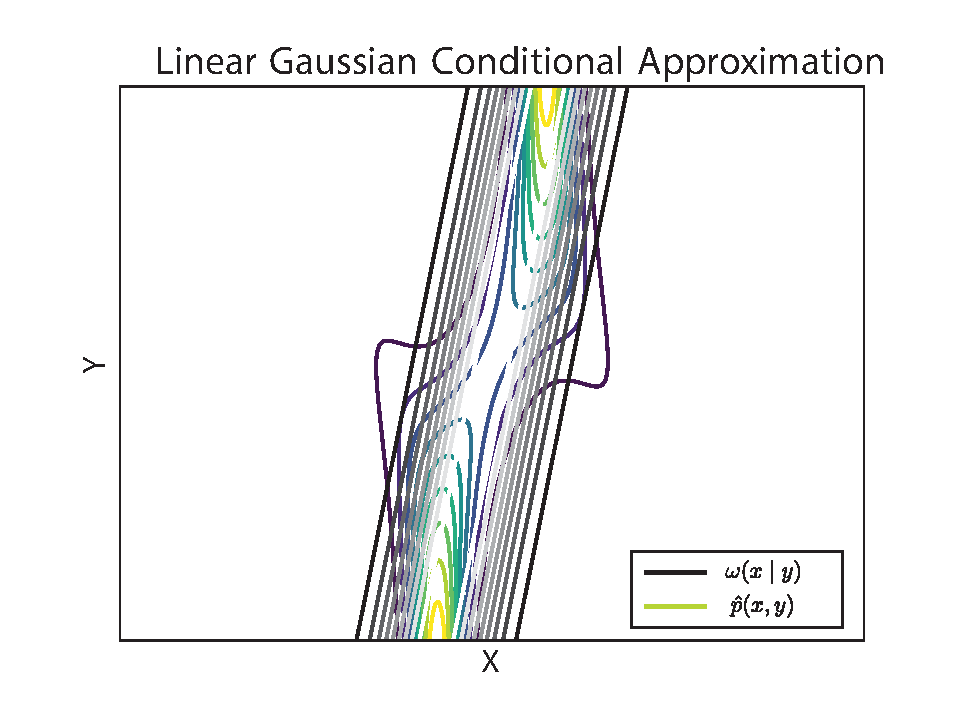
\includegraphics[width=0.4\textwidth]{linear_approx}

%%   \vspace{-5mm}\caption{\small VIP optimizes a lower bound on MI
%%   w.r.t.~a distribution $\omega(x\mid y)$ approximating the
%%   conditional $\hat{p}(x\mid y)$. We use a linear Gaussian
%%   approximation in this case.  }  
%% \end{figure} 

Optimization of the bound~\eqref{eq:varmi_approx} with respect to the
auxiliary distribution $\omega(x\mid y)$ can be complicated in
general.  In this section we consider optimization for the class of
auxiliary distributions which are in the exponential family, when
conditioned on a hypothesized measurement.  This flexible family
allows for nonlinear dependence on the observation $y$ as illustrated
in \FIG\ref{fig:approx} (right).  We show that the resulting
optimization is convex in the exponential family natural parameters
and that optimality conditions yield a relaxation of the moment
matching property for exponential families.

%% We represent conditional exponential families with natural parameters
%% that are themselves functions of the conditioning variable $y$.  With
%% a slight abuse of terminology, we refer to this as a \emph{link
%% function}.  This rich family of distributions is strictly larger than
%% the set of joint distributions $\omega(x,y)$ in the exponential
%% family, and thus allows tighter achievable bounds.  We conclude by
%% characterizing the optimization of link function parameters.


\subsection{Optimizing the Auxiliary Distribution}

Consider the set of conditional distributions in the exponential
family having density,
\begin{equation}
  \omega_\theta(x \mid y) = h(x)\exp\left( \theta(y)^T \phi(x,y) - A(\theta(y)) \right),
\end{equation}
with natural parameters $\theta(y)$ a function of the conditioning
variable, sufficient statistics $\phi(x,y)$, base measure $h(x)$ and
log-partition function $A(\theta(y))$.  Optimizing the bound
in \EQN\eqref{eq:varmi_approx} is equivalent to minimizing the cross
entropy,
\begin{equation}\label{eq:crossent}
  \theta^{*}(y) = \argmin_{\theta} J(\theta) \equiv \EE_{\hat{p}}[ - \log \omega_{\theta}(x \mid y) ].
\end{equation}
Convexity of $J(\theta)$ can be established by explicit calculation of
the Hessian.  Alternatively, by adding a constant \mbox{$-H(\hat{p})$}
we have the following problem, which is equivalent to $J(\theta)$ up
to constant terms,
\begin{equation}\label{eq:dual}
  \theta^*(y) = \argmin_\theta \EE_{\hat{p}_y}\left[ \KL{\hat{p}_{x\mid y}}{\omega_\theta} \right]
\end{equation}
For brevity we have introduced the shorthand \mbox{$\hat{p}_{x\mid
y} \equiv
\hat{p}(x\mid y)$}.  For any realization $Y=y$ the KL term is convex in
$\theta(y)$, a well known property of the exponential
families~\citep{wainwright_jordan}.  \EQN\eqref{eq:dual} is then a
convex combination of convex functions, thus convexity holds.

The optimal parameter function $\theta^{*}(y)$ is given by the
stationary point condition,
\begin{equation}\label{eq:stationary_point}
  \EE_{\hat{p}_y}\left[ \EE_{\omega_{\theta^{*}}}[ \phi(x,y) \mid Y=y ] \right] = \EE_{\hat{p}}[\phi(x,y)].
\end{equation}
This is a weaker condition than the standard moment matching property
of exponential families, which typically minimizes KL.
Under~\eqref{eq:stationary_point} moments of $\omega(x\mid y)$ must
match \emph{in expectation} w.r.t.~the marginal distribution $p(y)$,
but need not be equal for any particular realization $Y=y$.

%% \begin{gather}
%%   \omega(X \mid Y = y; \theta) = \exp\left( \theta(y)^T \phi(X) -
%%     A(\theta(y)) \right) \\
%%   A(\theta(y)) = \log \int_{\Xcal \times \Ycal} \!\!\!\!\!\exp\left( \theta(y)^T \phi(x) \right)
%% dx dy
%% \end{gather}

\subsection{Parameter Function Optimization}

Stationary conditions~\eqref{eq:stationary_point} are in terms of a
function $\theta(y)$ which is assumed to be parametric.  Let $\eta$ be
parameters of the function, denoted $\theta_{\eta}(y)$.  Stationary
conditions in terms of parameters $\eta$ are then,
\begin{equation*}
  \EE_{p_y}\left[ \left( D_\eta \theta \right)^T \EE_{\omega_\eta}[\phi(x,y)]
    \right]
    \!= \EE_{p_y}\left[ \left( D_\eta \theta \right)^T \EE_{p_{x\mid
          y}}[ \phi(x,y) ] \right]
\end{equation*}
where $D_\eta \theta$ is the Jacobian matrix of partial derivatives.
If $\theta(y)$ is convex in the parameters $\eta$ then the
optimization \EQN\eqref{eq:dual} remains convex.

In principle, the map $\theta_{\eta}(y)$ can be any parametric
function, for example a neural network with parameters $\eta$.
Indeed, in related work~\cite{chen2018learning} optimize the MI
bound~\eqref{eq:varmi} w.r.t.~a neural network map for feature
selection tasks.  However, such an approach violates the convexity
properties above and leads to computation that is prohibitive for
sequential decision making tasks.

%% One approach is to
%% represent $\theta_{\eta}(y)$ as a neural network, with parameters
%% $\eta$.  In this setting, the Jacobian can be efficiently calculated
%% for any $y$ via backpropagation.

